\documentclass[12pt]{report}
\usepackage[utf8]{inputenc}
\usepackage[english, russian]{babel}
\usepackage{fontspec} 
\usepackage[14pt]{extsizes}
\usepackage{caption}
\usepackage{graphicx}
\usepackage[left=2cm, right=2cm, top=1cm, bottom=2.5cm]{geometry}
\usepackage{listings}
\usepackage{titlesec, blindtext, color} % подключаем нужные пакеты
\usepackage{setspace} % полуторный интервал
\usepackage{hyperref}
\definecolor{gray75}{gray}{0.75} % определяем цвет
\newcommand{\hsp}{\hspace{20pt}} % длина линии в 20pt
% titleformat определяет стиль
\titleformat{\chapter}[hang]{\Huge\bfseries}{\thechapter\hsp\textcolor{gray75}\hsp}{0pt}{\Huge\bfseries}

% Для листинга кода:
\lstset{ 
	language=[Sharp]C,                 % выбор языка для подсветки (здесь это С)
	basicstyle=\small\sffamily, % размер и начертание шрифта для подсветки кода
	numbers=left,               % где поставить нумерацию строк (слева\справа)
	numberstyle=\tiny,           % размер шрифта для номеров строк
	stepnumber=1,                   % размер шага между двумя номерами строк
	numbersep=5pt,                % как далеко отстоят номера строк от подсвечиваемого кода
	showspaces=false,            % показывать или нет пробелы специальными отступами
	showstringspaces=false,      % показывать или нет пробелы в строках
	showtabs=false,             % показывать или нет табуляцию в строках
	frame=single,              % рисовать рамку вокруг кода
	tabsize=2,                 % размер табуляции по умолчанию равен 2 пробелам
	captionpos=t,              % позиция заголовка вверху [t] или внизу [b] 
	breaklines=true,           % автоматически переносить строки (да\нет)
	breakatwhitespace=false, % переносить строки только если есть пробел
}
\defaultfontfeatures{Ligatures={TeX},Renderer=Basic} 
\setmainfont[Ligatures={TeX,Historic}]{Times New Roman}
\begin{document}
	
	%\def\chaptername{} % убирает "Глава"
	\begin{titlepage}
		\begin{table}[ht]
			\centering
			\begin{tabular}{|c|p{420pt}|} 
				\hline
				\begin{tabular}[c]{@{}c@{}} 
\includegraphics[scale=0.37]{source/EmblemBMSTU} \\\end{tabular} &
				\footnotesize\begin{tabular}[c]{@{}c@{}}\textbf{Министерство~науки~и~высшего~образования~Российской~Федерации}\\\textbf{Федеральное~государственное~бюджетное~образовательное~учреждение}\\\textbf{~высшего~образования}\\\textbf{«Московский~государственный~технический~университет}\\\textbf{имени~Н.Э.~Баумана}\\\textbf{(национальный~исследовательский~университет)»}\\\textbf{(МГТУ~им.~Н.Э.~Баумана)}\\\end{tabular}  \\
				\hline
			\end{tabular}
		\end{table}
		\noindent\rule{\textwidth}{4pt}
		\noindent\rule[14pt]{\textwidth}{1pt}
		\hfill 
		\noindent
		\makebox{ФАКУЛЬТЕТ~}%
		\makebox[\textwidth][l]{\underline{~~~~«Информатика и системы управления»~~~~~~~~~~~~~~~~~~~~~~~~~~~~~~~~~~~~~~~~~~~~}}%
		\\
		\noindent
		\makebox{КАФЕДРА~}%
		\makebox[\textwidth][l]{\underline{~~~~~~~«Программное обеспечение ЭВМ и информационные технологии»~~~~~~~~}}%
		\\
		
		
		\begin{center}
			\vspace{3cm}
			{\bf\huge Отчёт\par}
			{\bf\Large по лабораторной работе № 1\par}
			\vspace{0.5cm}
		\end{center}
		
		
		\noindent
		\makebox{\large{\bf Название:}~~~}
		\makebox[\textwidth][l]{\large\underline{~Расстояния Левенштейна и Дамерау-Левенштейна~}}\\
		
		\noindent
		\makebox{\large{\bf Дисциплина:}~~~}
		\makebox[\textwidth][l]{\large\underline{~Анализ алгоритмов~}}\\
		
		\vspace{1.5cm}
		\noindent
		\begin{tabular}{l c c c c c}
			Студент      & ~ИУ7-55Б~               & \hspace{3.5cm} & \hspace{3.5cm}                 & &  Д.О. Склифасовский \\\cline{2-2}\cline{4-4} \cline{6-6} 
			\hspace{3cm} & {\footnotesize(Группа)} &                & {\footnotesize(Подпись, дата)} & & {\footnotesize(И.О. Фамилия)}
		\end{tabular}
		
		\vspace{1cm}
		
		\noindent
		\begin{tabular}{l c c c c}
			Преподователь & \hspace{6cm}   & \hspace{3.5cm}                 & & ~~~~~~ Л.Л. Волкова ~~~~~~\\\cline{3-3} \cline{5-5} 
			\hspace{3cm}  &                & {\footnotesize(Подпись, дата)} & & {\footnotesize(И.О. Фамилия)}
		\end{tabular}
		
		\begin{center}	
			\vfill
			\large \textit {Москва, 2020}
		\end{center}
		
		\thispagestyle {empty}
		\pagebreak
	\end{titlepage}
	\restoregeometry
	
	\tableofcontents
	\onehalfspacing
	\newpage
	\chapter*{Введение}
	\addcontentsline{toc}{chapter}{Введение}
	
	\textbf{Редакионное расстояние} или \textbf{расстояние Левенштейна} - это минимальное количество редакторских операций, которые необходимы для преобразования одной строки в другую.
	
	Расстояние Левенштейна и его обобщения активно применяются: 
	\begin{enumerate}
		\item[1)] для исправления ошибок в слове (в поисковых системах, базах данных, при вводе текста, при автоматическом распознавании отсканированного текста или речи);
		\item[2)] для сравнения текстовых файлов утилитой diff и ей подобными. Здесь роль «символов» играют строки, а роль «строк» — файлы;
		\item[3)] в биоинформатике для сравнения генов, хромосом и белков.
	\end{enumerate}
	
	Целью данной лабораторной работы является реализовать и сравнить по эффективности алгоритмы поиска расстояний Левенштейна и Дамерау-Левенштейна.
	
	Задачи данной лабораторной работы:
	\begin{enumerate}
		\item[1)] дать математическое описание расстояний;
		\item[2)] разработать алгоритмы поиска расстояний;
		\item[3)] реализовать алгоритмы поиска расстояний;
		\item[4)] провести эксперименты по замеру времени работы реализации алгоритмов;
		\item[5)] провести сравнительный анализ реализаций алгоритмов по затрачиваемому времени (и максимально затрачиваемой памяти);
		\item[6)] дать теоретическую оценку максимально затрачиваемых по памяти реализациям алгоритмов.
	\end{enumerate}
	
	\chapter{Аналитическая часть} 
	В данном разделе представлено математическое описание расстояний.
	\section{Алгоритм Левенштейна}
	Задача по нахождению расстояния Левенштейна заключается в поиске минимального количества операций вставки/удаления/замены для превращения одной строки в другую.
	
	\textbf{Редакционные операции:}
	\begin{enumerate}
		\item[1)] вставки (I, insert) штраф 1;
		\item[2)] удаления (D, delete) штраф 1;
		\item[3)] замена (R, replace) штраф 1;
		\item[4)] совпадение (M, match) штраф 0.
	\end{enumerate}
	
	Пусть $S_{1}$ и $S_{2}$ — две строки (длиной M и N соответственно) над некоторым алфавитом, тогда расстояние Левенштейна можно подсчитать по следующей формуле:
	
	\begin{equation}
		D(i,j) = \left\{ \begin{array}{l | l}
			0, & \textrm{$i = 0, j = 0$}\\
			i, & \textrm{$j = 0, i > 0$}\\
			j, & \textrm{$i = 0, j > 0$}\\
			min(D(i,j-1)+1\\
				D(i-1, j) +1,\\
				D(i-1, j-1) + m(S_{1}[i], S_{2}[j])\\
				), &\textrm{$j>0, i>0$}
		\end{array} \right.
	\end{equation}
	где $m(a, b)$ равна 1, если $a$ не равно $b$ и 0 иначе; $min(a, b, c)$ возвращает минимальный аргумент.
	
	\section{Алгоритм Дамерау-Левенштейна}
	В алгоритме Дамерау-Левенштейна добавлена еще одна операция перестановки символа (X, exchange), штраф 1.
	
	\begin{equation}
		D(i,j) = \left\{ \begin{array}{l | l}
			0, & \textrm{$i = 0, j = 0$}\\
			i, & \textrm{$j = 0, i > 0$}\\
			j, & \textrm{$i = 0, j > 0$}\\
			min(\\D(i,j-1)+1,\\
			D(i-1, j) +1, &\textrm{$j>0, i>0$}\\
			D(i-1, j-1) + m(S_{1}[i], S_{2}[j])\\
			D(i-2, j-2) + 1 &\textrm{if $i,j>1$ and} \\
			), & \textrm{$a_{i} = b_{j-1},a_{i-1}=b_{j} $}
		\end{array} \right.
	\end{equation}
	
	\newgeometry{pdftex, left=2cm, right=2cm, top=2.5cm, bottom=2.5cm}
	\chapter{Конструкторская часть}
	В данном разделе описаны схемы разработанных алгоритмов.
	\section{Разработка алгоритмов}
	
	На \hyperref[picture_1]{рисунке 1} изображена схема матричного алгоритма нахождения расстояний Левенштейна.
	\begin{figure}[h!]\label{picture_1}
		\center{\includegraphics[scale=0.55]{source/firstAlgorithm.png}}
		\caption*{Рисунок 1. Схема матричного алгоритма Левенштейна}
	\end{figure}
	\newpage
	На \hyperref[picture_2]{рисунке 2} изображена схема рекурсивного алгоритма нахождения расстояний Левенштейна.
	\begin{figure}[h!]\label{picture_2}
		\center{\includegraphics[scale=0.8]{source/secondAlgorithm.png}}
		\caption*{Рисунок 2. Схема рекурсивного алгоритма Левенштейна}
	\end{figure}
	\newpage
	На \hyperref[picture_3]{рисунке 3} изображена схема рекурсивного алгоритма с использованием матрицы нахождения расстояний Левенштейна.
	\begin{figure}[h!]\label{picture_3}
		\center{\includegraphics[scale=0.8]{source/thirdAlgorithm.png}}
		\caption*{Рисунок 3. Схема рекурсивного алгоритма Левенштейна с использованием матрицы}
	\end{figure}
	\newpage
	На \hyperref[picture_4]{рисунке 4} изображена схема матричного алгоритма нахождения расстояний Дамерау-Левенштейна.
	\begin{figure}[h!]\label{picture_4}
		\center{\includegraphics[scale=0.8]{source/fourthAlgorithm.png}}
		\caption*{Рисунок 4. Схема матричного алгоритма Дамерау-Левенштейна}
	\end{figure}
	\restoregeometry
	
	\newpage
	\onehalfspacing
	\section{Сравнительный анализ памяти}
	\subsection{Матричная реализация}
	В случае \textit{матричной реализации} алгоритма нужно хранить:
	\begin{enumerate}
		\item матрица: $C_{1} * (lenFirstStr + 1) + (lenFirstStr + 1) * C_{1} * (lenSecondStr + 1)$;
		\item переменная ($isNotEqual$): $C_{2}$;
		\item счетчики: $2C_{2}$.
	\end{enumerate}
	Также нужно передать параметры $C_{2} * len$.
	
	\noindent Таким образом, размер запрашиваемой памяти равен: $C_{1} * (lenFirstStr + 1) + (lenFirstStr + 1) * C_{1} * (lenSecondStr + 1) + C_{2} + 2C_{2} + C_{2} * len$.
	
	\subsection{Рекурсивная реализация}
	В случае \textit{рекурсивной реализации} алгоритма нужно хранить:
	\begin{enumerate}
		\item[1)] значения переменных: $4C_{2}$;
		\item[2)] также нужно передать параметры $C_{2} * len$.
	\end{enumerate}
	
	\noindent Таким образом, размер запрашиваемой памяти равен:
	$C_{2} + C_{2} * len$
	
	\subsection{Вывод}
	Память матричного алгоритма растет пропорционально их произведения длин двух строк, а в случае рекурсивного алгоритма, она растет пропорционально сумме длин строк. Таким образом, на строках большей длины преимущество будет иметь рекурсивный алгоритм.
	
	
	\newpage
	\chapter{Технологическая часть}
	В данной части даны общие требования к программе, средства реализации и реализация алгоритмов
	\section{Общие требования}
	\noindent\textbf{Требования к вводу:}
	\begin{enumerate}
		\item[1)] выбирается какой алгоритм (из 4) будет использоваться: 
		\begin{enumerate}
			\item[1.1)] нерекурсивный алгоритм поиска расстояния Левенштейна с заполнением матрицы;
			\item[1.2)] рекурсивный алгоритм поиска расстояния Левенштейна без заполнения матрицы;
			\item[1.3)] рекурсивный алгоритм поиска расстояния Левенштейна с заполнением матрицы;
			\item[1.4)] нерекурсивный алгоритм поиска расстояния Дамерау-Левенштейна с заполнением матрицы.
		\end{enumerate}
		\item[2)] на вход подаются две строки;
		\item[3)] на выходе программа выводит значение расстояния между ними;
		\item[4)] в случае вызова матричного алгоритма программа выводит матрицу;
		\item[5)] также необходимо предусмотреть выполнение замеров процессорного времени для каждого алгоритма.
	\end{enumerate}
	
	\noindent\textbf{Требования к программе:}
	\begin{enumerate}
		\item[1)] две пустые строки являются корректным вводом; 
		\item[2)] uppercase и lowcase буквы считаются разными.
	\end{enumerate}
	
	\section{Средства реализации}
	В качестве языка программирования был выбран С\#, так как он объектный, достаточно быстрый и в нем можно легко писать код, а требований по конкретнему языку не выдвигалось.\hyperref[literature]{[1]}
	\par Среда разработки - Visual Studio.\hyperref[literature]{[2]}
	
	Для замеров процессорного времени используется функция $Stopwatch$.\hyperref[literature]{[3]}
	 
	\section{Реализация алгоритмов}
	\begin{lstlisting}[label=sone-code,caption=Функция нахождения минимума из 3 переменных]
		private static int Min(int first, int second, int third)
		{
			int[] arr = { first, second, third };
			return arr.Min();
		}
	\end{lstlisting}
	\begin{lstlisting}[label=some-code,caption=Функция нахождения расстояния Левенштейна используя матрицу]
		public static int LevTable(string firstStr, string secondStr)
		{
			int lenFirstStr = firstStr.Length + 1;
			int lenSecondStr = secondStr.Length + 1;
			
			int[,] table = new int[lenFirstStr, lenSecondStr];
			for (int i = 0; i < lenFirstStr; i++)
			for (int j = 0; j < lenSecondStr; j++) { table[i, j] = i + j; }
			
			int isNotEqual = 1;
			for (int i = 1; i < lenFirstStr; i++)
			{
				for (int j = 1; j < lenSecondStr; j++)
				{
					if (firstStr[i - 1] == secondStr[j - 1]) { isNotEqual = 0; }
					table[i, j] = Min(table[i - 1, j] + 1,
					table[i, j - 1] + 1,
					table[i - 1, j - 1] + isNotEqual);
					isNotEqual = 1;
				}
			}
			return table[lenFirstStr - 1, lenSecondStr - 1];
		}
	\end{lstlisting}
	\begin{lstlisting}[label=sone-code,caption=Функция нахождения расстояния Левенштейна рекурсивно]
		public static int LevRecursion(string firstStr, string secondStr)
		{
			if (firstStr == "" || secondStr == "") { return Math.Abs(firstStr.Length - secondStr.Length); }
			int isNotEqual = 1;
			if (firstStr[firstStr.Length - 1] == secondStr[secondStr.Length - 1]) { isNotEqual = 0; }
			return Min(LevRecursion(firstStr, secondStr.Substring(0, secondStr.Length - 1)) + 1,
			LevRecursion(firstStr.Substring(0, firstStr.Length - 1), secondStr) + 1,
			LevRecursion(firstStr.Substring(0, firstStr.Length - 1), secondStr.Substring(0, secondStr.Length - 1)) + isNotEqual);
		}
	\end{lstlisting}
	\begin{lstlisting}[label=sone-code,caption=Функции нахождения расстояния Левенштейна рекурсивно с использованием матрицы]
		private static int GetMinValue(int[,] table, string first, string second, int lenFirst, int lenSecond)
		{
			int isNotEqual = (first[lenFirst - 1] == second[lenSecond - 1]) ? 0 : 1;
			int firstParam = FindLevDistance(table, first, second.Substring(0, lenSecond - 1)) + 1;
			int secondParam = FindLevDistance(table, first.Substring(0, lenFirst - 1), second) + 1;
			int thirdParam = FindLevDistance(table, first.Substring(0, lenFirst - 1), second.Substring(0, lenSecond - 1)) + isNotEqual;
			return Min(firstParam, secondParam, thirdParam);
		}
		
		private static int FindLevDistance(int[,] table, string first, string second)
		{
			int lenFirst = first.Length;
			int lenSecond = second.Length;
			
			if (lenFirst == 0 || lenSecond == 0)
			{
				table[lenFirst, lenSecond] = Math.Abs(lenFirst - lenSecond);
				return table[lenFirst, lenSecond];
			}
			
			if (table[lenFirst, lenSecond] == -1)
			table[lenFirst, lenSecond] = GetMinValue(table, first, second, lenFirst, lenSecond);
			return table[lenFirst, lenSecond];
		}
		
		public static int LevTableRec(string firstStr, string secondStr)
		{
			int lenFirstStr = firstStr.Length + 1;
			int lenSecondStr = secondStr.Length + 1;
			int[,] table = new int[lenFirstStr, lenSecondStr];
			for (int i = 0; i < lenFirstStr; i++)
			for (int j = 0; j < lenSecondStr; j++) { table[i, j] = -1; }
			
			int res;
			if (lenFirstStr - 1 == 0 || lenSecondStr - 1 == 0)
			res = Math.Abs((lenFirstStr - 1) - (lenSecondStr - 1));
			else
			res = GetMinValue(table, firstStr, secondStr, lenFirstStr - 1, lenSecondStr - 1);
			
			Console.WriteLine("RecTable");
			for (int i = 0; i < lenFirstStr; i++)
			{
				for (int j = 0; j < lenSecondStr; j++) { Console.Write(String.Format("{0, 3}", table[i, j])); }
				Console.WriteLine();
			}
			
			return res;
		}
	\end{lstlisting}
	\begin{lstlisting}[label=sone-code,caption=Функция нахождения расстояния Дамерау-Левенштейна используя матрицу]
		public static int LevDamTable(string firstStr, string secondStr)
		{
			int lenFirstStr = firstStr.Length + 1;
			int lenSecondStr = secondStr.Length + 1;
			
			int[,] table = new int[lenFirstStr, lenSecondStr];
			for (int i = 0; i < lenFirstStr; i++)
			for (int j = 0; j < lenSecondStr; j++) { table[i, j] = i + j; }
			
			int isNotEqual = 1;
			for (int i = 1; i < lenFirstStr; i++)
			{
				for (int j = 1; j < lenSecondStr; j++)
				{
					if ((i > 1 && j > 1) && firstStr[i - 1] == secondStr[j - 2] && firstStr[i - 2] == secondStr[j - 1])
					table[i, j] = Math.Min(table[i, j], table[i - 2, j - 2] + 1);
					else
					{
						if (firstStr[i - 1] == secondStr[j - 1]) { isNotEqual = 0; }
						table[i, j] = Min(table[i - 1, j] + 1,
						table[i, j - 1] + 1,
						table[i - 1, j - 1] + isNotEqual);
					}
					isNotEqual = 1;
				}
			}
			return table[lenFirstStr - 1, lenSecondStr - 1];
		}
	\end{lstlisting}

	\newpage
	\chapter{Экспериментальная часть}
	В данном разделе описаны примеры рабты программы, результаты работы программы и приведен сравнительный анализ времени работы каждого из алгоритмов.
	\section{Примеры работы программы}
	На \hyperref[picture_5]{рисунке 5} представлен пример вызова матричного алгоритма Левенштейна.
	\begin{figure}[h!]\label{picture_5}
		\center{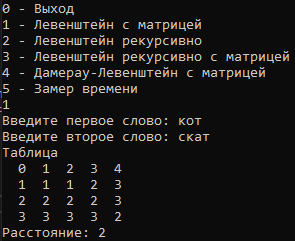
\includegraphics[scale=1]{source/Output1.png}}
		\caption*{Рисунок 5. Результат работы матричного алгоритма Левенштейна}
	\end{figure}
	\newpage
	\par На \hyperref[picture_6]{рисунке 6} представлен пример вызова рекурсивного алгоритма Левенштейна.
	\begin{figure}[h!]\label{picture_6}
		\center{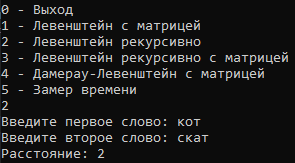
\includegraphics[scale=1]{source/Output2.png}}
		\caption*{Рисунок 6. Результат работы рекурсивного алгоритма Левенштейна}
	\end{figure}
	\par На \hyperref[picture_7]{рисунке 7} представлен пример вызова рекурсивного алгоритма Левенштейна с использованием матрицы.
	\begin{figure}[h!]\label{picture_7}
		\center{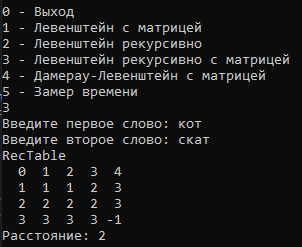
\includegraphics[scale=1]{source/Output3.png}}
		\caption*{Рисунок 7. Результат работы рекурсивного алгоритма Левенштейна с использованием матрицы}
	\end{figure}
	\newpage
	На \hyperref[picture_8]{рисунке 8} представлен пример вызова матричного алгоритма Дамерау-Левенштейна.
	\begin{figure}[h!]\label{picture_8}
		\center{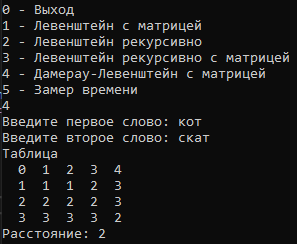
\includegraphics[scale=1]{source/Output4.png}}
		\caption*{Рисунок 8. Результат работы матричного алгоритма Дамерау-Левенштейна}
	\end{figure}

	%\restoregeometry
	\section{Результаты тестирования}
	\subsection{Результаты работы программы}
	Результаты тестирования программы приведены в \hyperref[table]{таблице 1}.
	
	\begin{table}[h]\label{table}
		\caption*{Таблица 1. Результаты работы программы}
		\begin{center}
			\begin{tabular}{|c c c|} 
				\hline
				Первое слово & Второе слово & Результат \\ [0.5ex] 
				\hline
				kot & skat & 2\\
				kot & skot & 1\\
				- & - & 0\\
				smth & something & 5\\
				something & osemthing & 3 | 2\\
				something & something & 0\\
				\hline
			\end{tabular}
		\end{center}
	\end{table}
	\onehalfspacing
	\subsection{Сравнительный анализ времени работы алгоритмов}
	Выполняется эксперимент. Берутся длина строк 2, 5, 10, 100, 200, 300, 500. Строки строятся рандомно. По \hyperref[picture_9]{рисунку 9 } можно увидеть, что самым долгим алгоритмом для строк большой длины является рекурсивный алгоритм без использования матрицы. Из-за того, что данный алгоритм выполняет много повторных операций, он намного дольше остальных. Самым быстрым является матричный алгоритм поиска расстояний Левенштейна. Длина строки влияет на работу данного алгоритма несущественно. Алгоритм Дамерау-Левенштейна немного медленнее, так как выполняется дополнительное сравнение в цикле. Рекурсивный алгоритм с использованием матрицы быстрее, чем обычный рекурсивный алгоритм, но медленнее матричных.
	\begin{figure}[h]\label{picture_9}
		\center{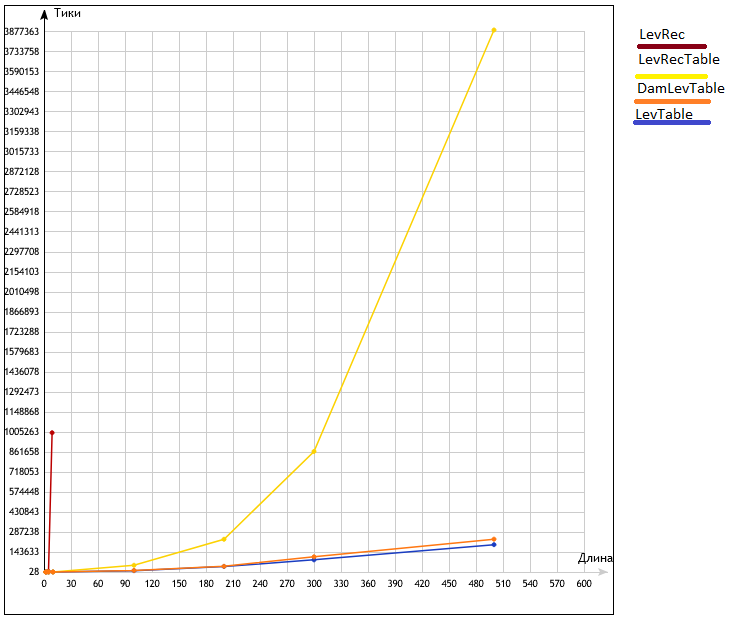
\includegraphics[scale=1]{source/graphs.png}}
		\caption*{Рисунок 9. Результат замера времени работы алгоритмов}
	\end{figure}
	\restoregeometry
	\onehalfspacing
	\chapter*{Заключение}
	\addcontentsline{toc}{chapter}{Заключение}
	В ходе лабораторной работы были разработаны и реализованы алгоритмы нахождения расстояния Левенштейна (матричный, рекурсивный, рекурсивный с использованием матрицы) и Дамерау-Левенштейна (матричный), а также был проведен анализ затрачиваемых ресурсов каждого из метода. В результате, после получения результата замера времени работы алгоритмов, было получено, что самым быстрым алгоритмом является матричный алгоритм нахождения расстояния Левенштейна, рекурсивный алгоритм оказался самым медленным, но рекурсивный алгоритм тратит меньше памяти, чем остальные.
	
	\newpage
	\chapter*{Литература}
	\addcontentsline{toc}{chapter}{Литература}
	\begin{enumerate}
		\label{literature}
		\item Документация по C\#. -URL: \href{https://docs.microsoft.com/ru-ru/dotnet/csharp/}{https://docs.microsoft.com/ru-ru/dotnet/csharp/} (дата обращения: 01.10.2020). -Текст: электронный.
		\item Документация по семейству продуктов Visual Studio. -URL:\par \href{https://docs.microsoft.com/ru-ru/visualstudio/?view=vs-2019}{https://docs.microsoft.com/ru-ru/visualstudio/?view=vs-2019 } (дата обращения: 01.10.2020). -Текст: электронный.
		\item Stopwatch Класс. -URL: \href{https://goo.su/2e99}{https://goo.su/2e99 } (дата обращения: 01.10.2020). -Текст: электронный.
		\item Под капотом у Stopwatch. -URL:  \href{https://habr.com/ru/post/226279/}{https://habr.com/ru/post/226279/} (дата обращения: 01.10.2020). Текст: электронный.
		\item Вычисление редакционного расстояния. -URL: \href{https://habr.com/ru/post/117063/}{https://habr.com/ru/post/117063/} (дата обращения: 01.10.2020). Текст: электронный.
	\end{enumerate}
\end{document}

